\setcounter{chapter}{14}
\chapter{Mécanique des fluides}

Dans toute cette leçon, le fluide est \trou{incompressible}. Sa masse volumique $\rho$ est une \trou{constante}. Elle ne dépend ni du point du fluide considéré ni du temps.
\section{Equilibre d'un fluide et d'un objet immergé}
\subsection{Statique des fluides (rappels)}

A chaque point M d'un fluide, on peut associer une pression P qui se mesure en \trou{pascal} (Pa).
Sous l'effet du champ de pesanteur $\overrightarrow{g}$, la pression d'un point  du fluide dépend de \trou{son altitude $z$}.

\etiquetterouge{On retient que}

\begin{minipage}{0.45\textwidth}
 $$\boxed{P_2- P_1 =\trou{ \rho g (z_1 - z_2)}}$$
 
 
Attention à \trou{l'orientation} de l'axe (Oz)
\end{minipage}
\hfill
\begin{minipage}{0.45\textwidth}
% Pattern Info
 
\tikzset{
pattern size/.store in=\mcSize, 
pattern size = 5pt,
pattern thickness/.store in=\mcThickness, 
pattern thickness = 0.3pt,
pattern radius/.store in=\mcRadius, 
pattern radius = 1pt}
\makeatletter
\pgfutil@ifundefined{pgf@pattern@name@_3ta6xpmll}{
\pgfdeclarepatternformonly[\mcThickness,\mcSize]{_3ta6xpmll}
{\pgfqpoint{0pt}{0pt}}
{\pgfpoint{\mcSize+\mcThickness}{\mcSize+\mcThickness}}
{\pgfpoint{\mcSize}{\mcSize}}
{
\pgfsetcolor{\tikz@pattern@color}
\pgfsetlinewidth{\mcThickness}
\pgfpathmoveto{\pgfqpoint{0pt}{0pt}}
\pgfpathlineto{\pgfpoint{\mcSize+\mcThickness}{\mcSize+\mcThickness}}
\pgfusepath{stroke}
}}
\makeatother
\tikzset{every picture/.style={line width=0.75pt}} %set default line width to 0.75pt        

\begin{tikzpicture}[x=0.75pt,y=0.75pt,yscale=-1,xscale=1]
%uncomment if require: \path (0,300); %set diagram left start at 0, and has height of 300

%Straight Lines [id:da1431580915407349] 
\draw    (100,280) -- (100,52) ;
\draw [shift={(100,50)}, rotate = 90] [color={rgb, 255:red, 0; green, 0; blue, 0 }  ][line width=0.75]    (10.93,-3.29) .. controls (6.95,-1.4) and (3.31,-0.3) .. (0,0) .. controls (3.31,0.3) and (6.95,1.4) .. (10.93,3.29)   ;
%Straight Lines [id:da19553928863883396] 
\draw    (90,250) -- (110,250) ;
%Straight Lines [id:da945394404180156] 
\draw    (90,120) -- (110,120) ;
%Straight Lines [id:da8594674598946904] 
\draw    (144,119.7) -- (157.4,119.7) ;
%Straight Lines [id:da7274688509203905] 
\draw    (150.7,127.2) -- (150.7,112.2) ;

%Straight Lines [id:da47087832586595935] 
\draw    (194.6,249.5) -- (208,249.5) ;
%Straight Lines [id:da7468781295482437] 
\draw    (201.3,257) -- (201.3,242) ;

%Straight Lines [id:da8920415703778027] 
\draw    (263.6,98.6) -- (263.6,155.4) ;
\draw [shift={(263.6,157.4)}, rotate = 270] [color={rgb, 255:red, 0; green, 0; blue, 0 }  ][line width=0.75]    (10.93,-3.29) .. controls (6.95,-1.4) and (3.31,-0.3) .. (0,0) .. controls (3.31,0.3) and (6.95,1.4) .. (10.93,3.29)   ;
%Shape: Rectangle [id:dp3919081166661982] 
\draw  [pattern=_3ta6xpmll,pattern size=19.799999999999997pt,pattern thickness=0.75pt,pattern radius=0pt, pattern color={rgb, 255:red, 0; green, 0; blue, 0}] (103.6,68.6) -- (309.8,68.6) -- (309.8,294.2) -- (103.6,294.2) -- cycle ;

% Text Node
\draw (95.8,30.4) node [anchor=north west][inner sep=0.75pt]    {$z$};
% Text Node
\draw (68.8,108.4) node [anchor=north west][inner sep=0.75pt]    {$z_{1}$};
% Text Node
\draw (68,238.8) node [anchor=north west][inner sep=0.75pt]    {$z_{2}$};
% Text Node
\draw (159.6,111.8) node [anchor=north west][inner sep=0.75pt]    {$M_{1}$};
% Text Node
\draw (211.2,240.8) node [anchor=north west][inner sep=0.75pt]    {$M_{2}$};
% Text Node
\draw (270.4,114) node [anchor=north west][inner sep=0.75pt]    {$\vec{g}$};
% Text Node
\draw (133.2,273.4) node [anchor=north west][inner sep=0.75pt]   [align=left] {fluide à l'équilibre};


\end{tikzpicture}
\end{minipage}

\subsection{Solide totalement immergé dans un liquide}


\begin{minipage}{0.45\textwidth}
	
\tikzset{every picture/.style={line width=0.75pt}} %set default line width to 0.75pt        

\begin{tikzpicture}[x=0.75pt,y=0.75pt,yscale=-1,xscale=1]
%uncomment if require: \path (0,300); %set diagram left start at 0, and has height of 300

%Straight Lines [id:da1431580915407349] 
\draw    (100,290) -- (100,36) ;
\draw [shift={(100,34)}, rotate = 90] [color={rgb, 255:red, 0; green, 0; blue, 0 }  ][line width=0.75]    (10.93,-3.29) .. controls (6.95,-1.4) and (3.31,-0.3) .. (0,0) .. controls (3.31,0.3) and (6.95,1.4) .. (10.93,3.29)   ;
%Straight Lines [id:da19553928863883396] 
\draw    (90,263.6) -- (110,263.6) ;
%Straight Lines [id:da945394404180156] 
\draw    (90,94) -- (110,94) ;
%Straight Lines [id:da8920415703778027] 
\draw    (323.6,87.1) -- (323.6,143.9) ;
\draw [shift={(323.6,145.9)}, rotate = 270] [color={rgb, 255:red, 0; green, 0; blue, 0 }  ][line width=0.75]    (10.93,-3.29) .. controls (6.95,-1.4) and (3.31,-0.3) .. (0,0) .. controls (3.31,0.3) and (6.95,1.4) .. (10.93,3.29)   ;
%Shape: Rectangle [id:dp5373877667432289] 
\draw   (170,94) -- (280,94) -- (280,264) -- (170,264) -- cycle ;
%Straight Lines [id:da9508886392388277] 
\draw    (170,104) -- (188,104) ;
\draw [shift={(190,104)}, rotate = 180] [color={rgb, 255:red, 0; green, 0; blue, 0 }  ][line width=0.75]    (10.93,-3.29) .. controls (6.95,-1.4) and (3.31,-0.3) .. (0,0) .. controls (3.31,0.3) and (6.95,1.4) .. (10.93,3.29)   ;
%Straight Lines [id:da39799050739514663] 
\draw    (170,174) -- (198,174) ;
\draw [shift={(200,174)}, rotate = 180] [color={rgb, 255:red, 0; green, 0; blue, 0 }  ][line width=0.75]    (10.93,-3.29) .. controls (6.95,-1.4) and (3.31,-0.3) .. (0,0) .. controls (3.31,0.3) and (6.95,1.4) .. (10.93,3.29)   ;
%Straight Lines [id:da6014552387688628] 
\draw    (170,234) -- (208,234) ;
\draw [shift={(210,234)}, rotate = 180] [color={rgb, 255:red, 0; green, 0; blue, 0 }  ][line width=0.75]    (10.93,-3.29) .. controls (6.95,-1.4) and (3.31,-0.3) .. (0,0) .. controls (3.31,0.3) and (6.95,1.4) .. (10.93,3.29)   ;
%Straight Lines [id:da5653486083787891] 
\draw    (262,104) -- (280,104) ;
\draw [shift={(260,104)}, rotate = 0] [color={rgb, 255:red, 0; green, 0; blue, 0 }  ][line width=0.75]    (10.93,-3.29) .. controls (6.95,-1.4) and (3.31,-0.3) .. (0,0) .. controls (3.31,0.3) and (6.95,1.4) .. (10.93,3.29)   ;
%Straight Lines [id:da9278285507191912] 
\draw    (252,174) -- (280,174) ;
\draw [shift={(250,174)}, rotate = 0] [color={rgb, 255:red, 0; green, 0; blue, 0 }  ][line width=0.75]    (10.93,-3.29) .. controls (6.95,-1.4) and (3.31,-0.3) .. (0,0) .. controls (3.31,0.3) and (6.95,1.4) .. (10.93,3.29)   ;
%Straight Lines [id:da2529721799410396] 
\draw    (242,234) -- (280,234) ;
\draw [shift={(240,234)}, rotate = 0] [color={rgb, 255:red, 0; green, 0; blue, 0 }  ][line width=0.75]    (10.93,-3.29) .. controls (6.95,-1.4) and (3.31,-0.3) .. (0,0) .. controls (3.31,0.3) and (6.95,1.4) .. (10.93,3.29)   ;
%Straight Lines [id:da7895068034344014] 
\draw    (230,264) -- (230,216) ;
\draw [shift={(230,214)}, rotate = 90] [color={rgb, 255:red, 0; green, 0; blue, 0 }  ][line width=0.75]    (10.93,-3.29) .. controls (6.95,-1.4) and (3.31,-0.3) .. (0,0) .. controls (3.31,0.3) and (6.95,1.4) .. (10.93,3.29)   ;
%Straight Lines [id:da20361196168232487] 
\draw    (230,94) -- (230,112) ;
\draw [shift={(230,114)}, rotate = 270] [color={rgb, 255:red, 0; green, 0; blue, 0 }  ][line width=0.75]    (10.93,-3.29) .. controls (6.95,-1.4) and (3.31,-0.3) .. (0,0) .. controls (3.31,0.3) and (6.95,1.4) .. (10.93,3.29)   ;

% Text Node
\draw (95.8,14.4) node [anchor=north west][inner sep=0.75pt]    {$z$};
% Text Node
\draw (71,82.4) node [anchor=north west][inner sep=0.75pt]    {$z_{2}$};
% Text Node
\draw (68,252.4) node [anchor=north west][inner sep=0.75pt]    {$z_{1}$};
% Text Node
\draw (330.4,102.5) node [anchor=north west][inner sep=0.75pt]    {$\vec{g}$};
% Text Node
\draw (221,266.4) node [anchor=north west][inner sep=0.75pt]    {$\overrightarrow{F_{1}}$};
% Text Node
\draw (221,64.4) node [anchor=north west][inner sep=0.75pt]    {$\overrightarrow{F_{2}}$};


\end{tikzpicture}
\end{minipage}
\hfill
\begin{minipage}{0.45\textwidth}

Le système étudié est une boite immergée dans un fluide de masse volumique $\rho$. Le fluide exerce des forces de pression sur le système. 
Les forces de pression latérales s'\trou{équilibrent}. La force de pression sur la face supérieure $\overrightarrow{F_2}$ est plus faible que la force de pression qui s'exerce sur la face inférieure $\overrightarrow{F_1}$.

La résultante des forces de pression s'écrit: $$\trou{\overrightarrow{F_1}+\overrightarrow{F_2}}= \overrightarrow{F_p}$$
$\overrightarrow{F_p}$ est la poussée \trou{d'Archimède
}.
\end{minipage}

On note $S$ la surface du haut et du bas de l'objet immergé et  $h=z_2-z_1$ sa hauteur. $\vec{k}$ est un vecteur unitaire ascendant. Calculons les forces pressantes exercées par le fluide sur la boîte:
\begin{align*}
  \overrightarrow{F_1} &= P_1\times S \cdot \vec{k} \\
  \overrightarrow{F_2} &= \trou{P_2\times S \cdot (-\vec{k})} \\
  \overrightarrow{F_1}+ \overrightarrow{F_2} &= \trou{(P_1-P_2)S \ \vec{k}} = \overrightarrow{F_p}
\end{align*}
or  $P_1-P_2 = \trou{\rho gh}$ donc $$\overrightarrow{F_p}=\trou{\rho  gh \times S \ \vec{k}}$$

\blocrouge{Poussée d'Archimède}{C'est la somme des forces exercées par un fluide sur la partie immergée d'un corps (solide ou liquide). Elle a pour valeur l'opposé du poids du fluide déplacé par ce corps. Mathématiquement $$\overrightarrow{F_p}= \trou{- \rho_{fluide}\times V_{immerge}\times \vec{g}}$$}


\begin{minipage}{0.55\textwidth}
\etiquettebleue{Expérience} 
	On accroche une masse à un dynamomètre, on mesure son poids: P. Puis, on immerge la masse dans une éprouvette graduée contenant de l'eau. La valeur indiquée par le dynamomètre diminue et vaut $P'$. 
	\begin{enumerate}
		\item Que vaut l'intensité de la poussée d'Archimède ?
		\item Cette valeur est-elle en accord avec la valeur prévue par la théorie ?
	\end{enumerate}
\end{minipage}
\hfill
\begin{minipage}{0.35\textwidth}
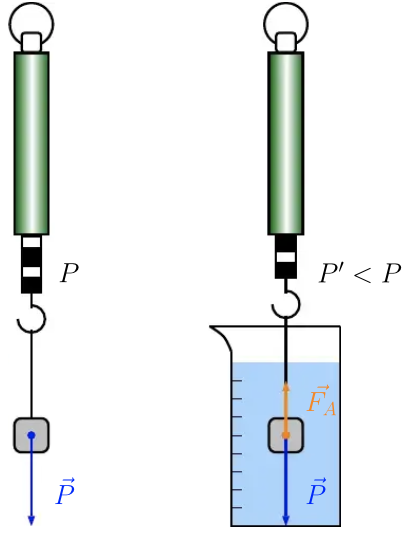
\includegraphics[scale=.4]{figures/archimede}
\end{minipage}


\section{Débit volumique}
\subsection{Régime permanent dans un tube}

\blocrouge{Définition}{Un régime permanent ou stationnaire signifie que les grandeurs physiques sont indépendantes du temps. Ici, la vitesse en un point M du fluide est constante au cours du temps.}

\etiquette{Signification} Le volume $V$ de fluide qui traverse une section pendant une durée $\Delta t$ correspond à un débit volumique $D$ $$D=\trou{\frac{V}{\Delta t}}$$

\etiquette{Exemples} 
\begin{itemize}
	\item Le débit sanguin circulant au travers de son coeur est de 5 L par minute. (à la maison convertir en mètre cube par seconde)
	\item Débit de la Seine: \SI{250}{\metre \cubed \per\second}
	\item Débit de l'eau au robinet \SI{e-3}{\metre \cubed \per\second}
\end{itemize}


\etiquette{Remarque} D'un point à un autre point du fluide la vitesse pourra changer. Voir exemple du tuyau pincé ci-après.

\subsection{Expression du débit volumique}
\begin{minipage}{.55\textwidth}
\begin{itemize}
	\item Où sont les particules de fluide qui vont traverser la section S entre les instants t=0 et t=$\Delta t$ ?
	\item La dernière particule de fluide à passer se situe à t=0 à une distance \trou{$l$ en amont de S} telle que $$l=\trou{v\times \Delta t}$$ 
	\item Le volume V s'écrit $\trou{l\times S}= \trou{v \times S \times \Delta t}$ 
\end{itemize}	
\end{minipage}
\hfill
\begin{minipage}{.40\textwidth}
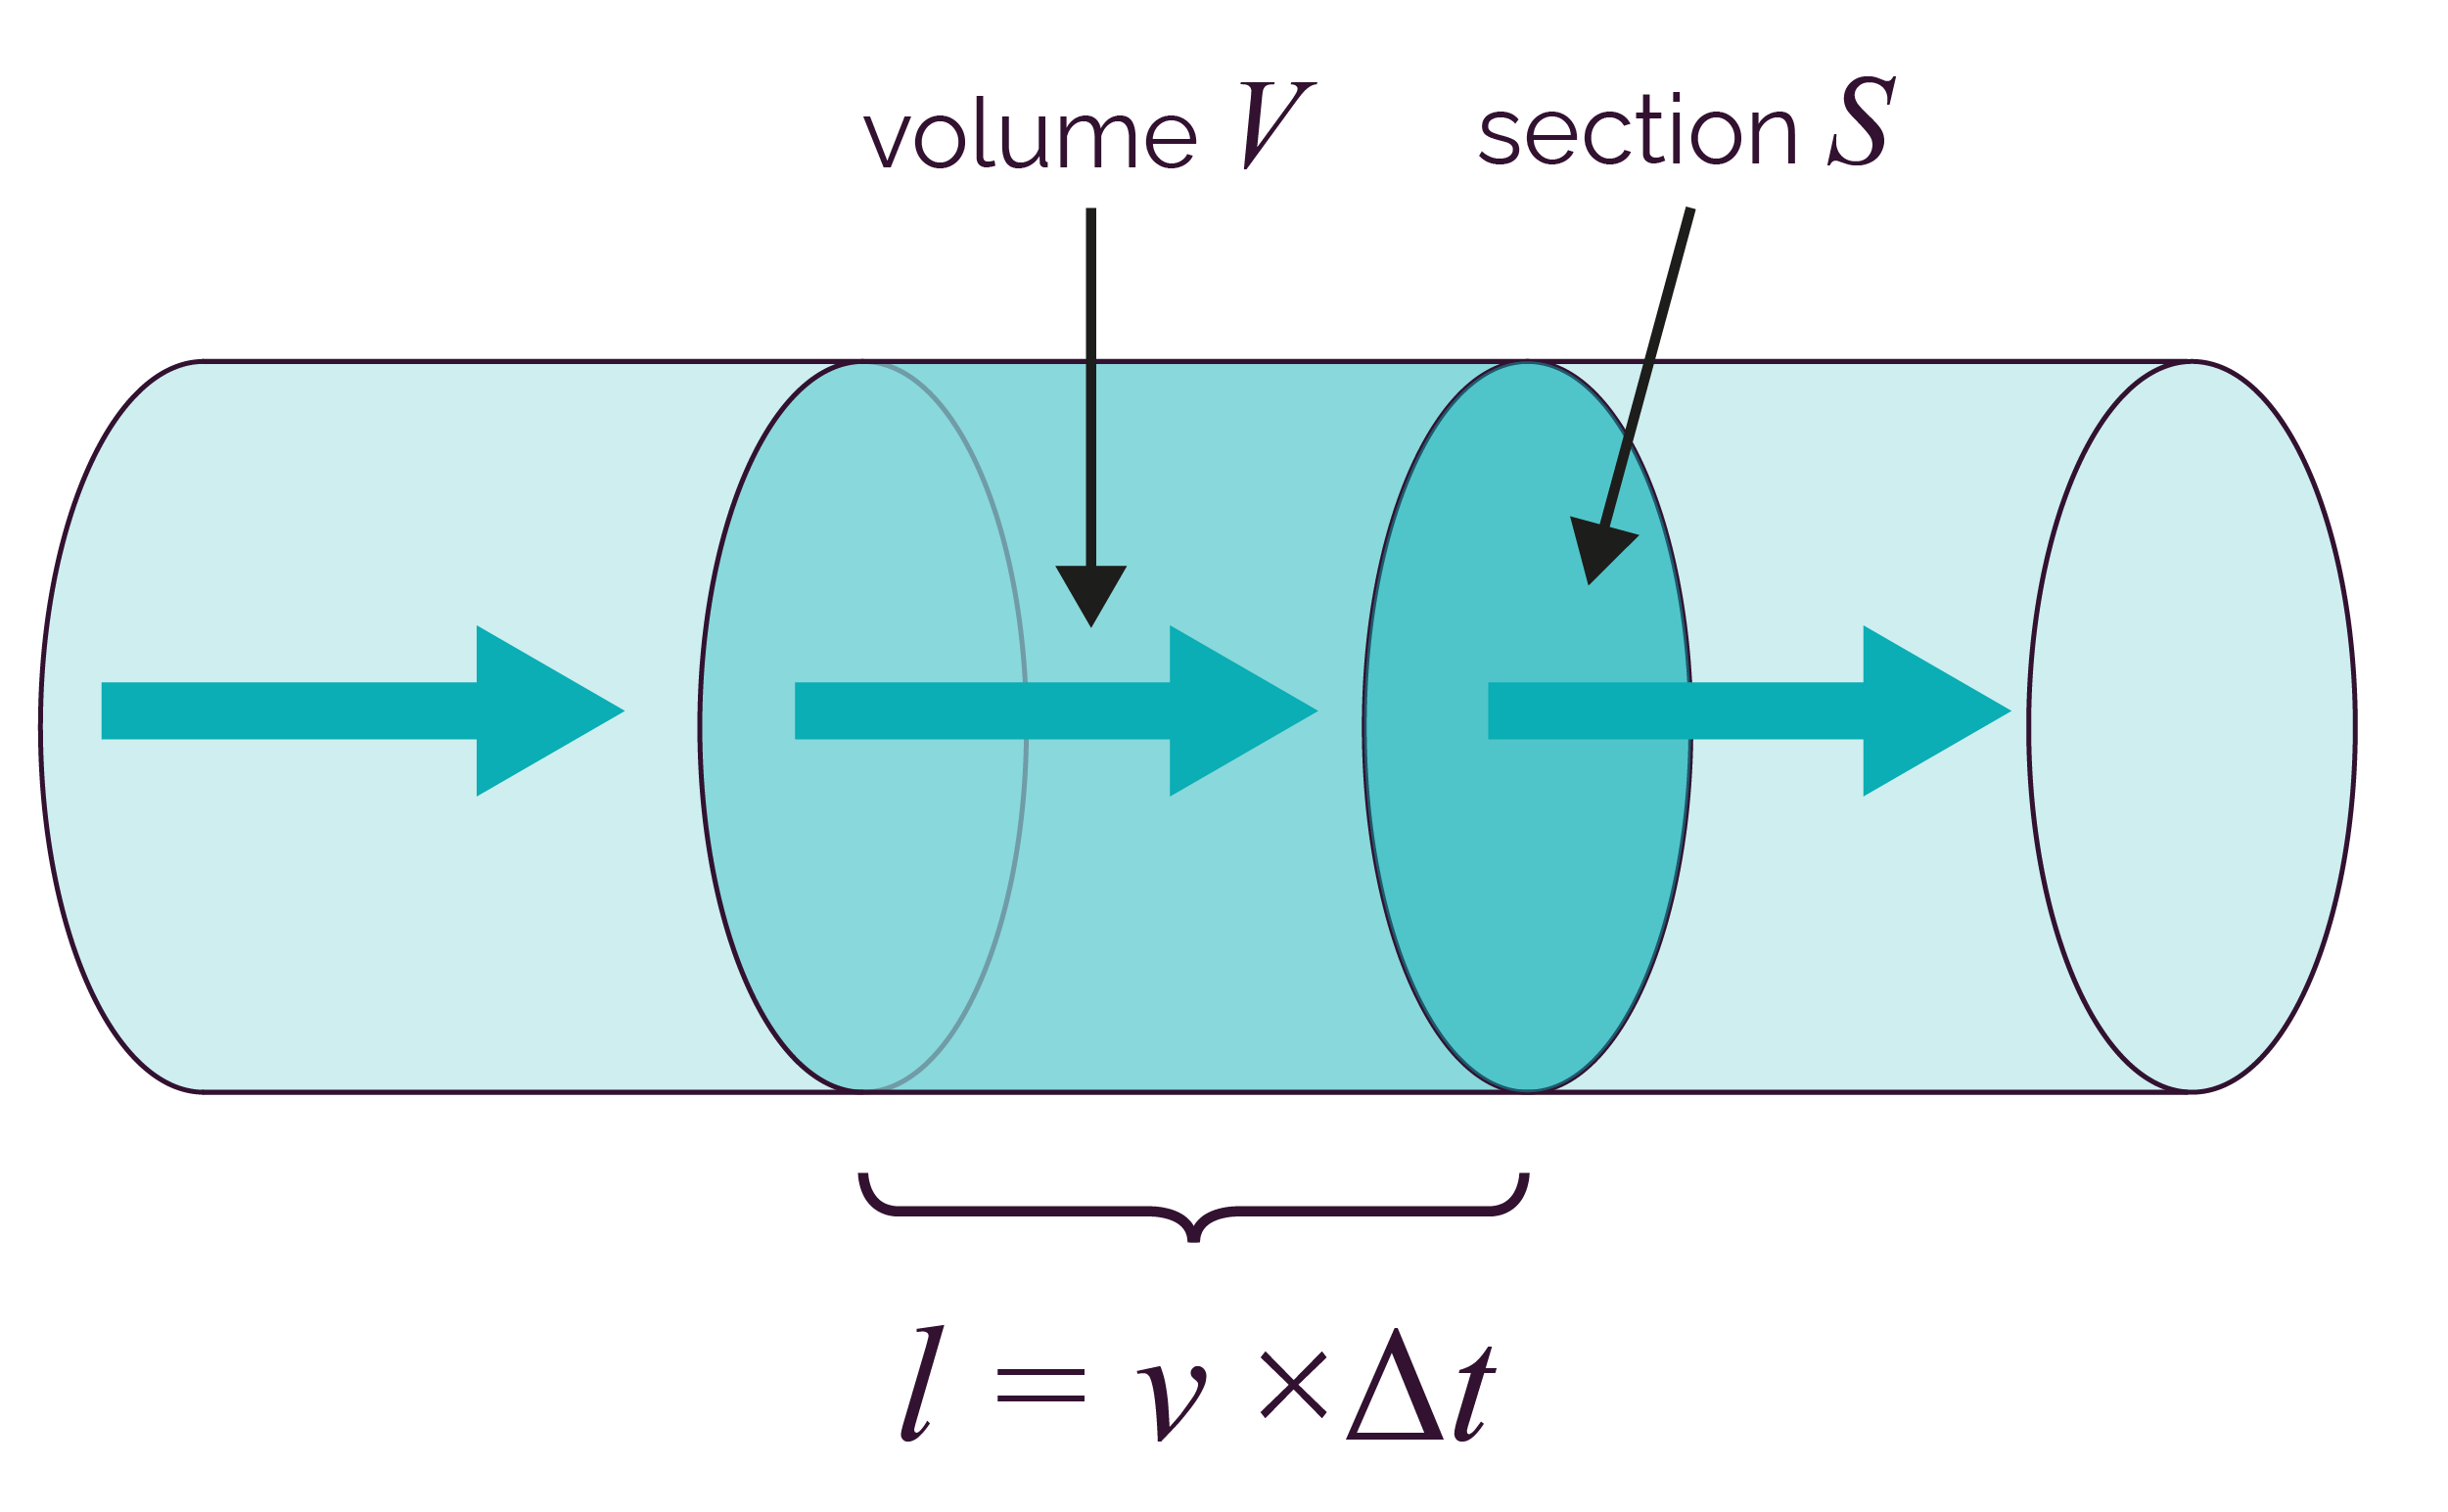
\includegraphics[scale=.3]{figures/debit_volumique}	
\end{minipage}


\blocrouge{A retenir}{Le débit volumique D est relié à la vitesse d'écoulement du fluide à travers une section S selon:$$D=\trou{S\times v}$$
D en \si{\metre \cubed \per \second } ; S en \si{\metre \squared} et $v$ en \si{\metre \per \second}}

\subsection{Conservation du débit}

\begin{minipage}{.50\textwidth}
En régime permanent le débit D se conserve.

 Observons le volume V de fluide qui traverse $S_1$ pendant $\Delta t$. Dans le même temps, le même volume traverse $S_2$.  
\end{minipage}
\hfill
\begin{minipage}{.45\textwidth}
\includegraphics[width=1\textwidth]{figures/consv_debit}
\end{minipage}

$$V=\trou{ S_1 \ell_1} = \trou{S_2 \ell_2}$$ 

\begin{align*}
	\ell_1 &= \trou{v_1} \times \Delta t\\
	\ell_2 &= \trou{v_2} \times \Delta t\\
\end{align*}

donc $$\boxed{D =\trou{S_1v_1} =\trou{S_2 v_2}=cste}$$

\blocgris{Application}{ Le débit d'un tuyau d'arrosage vaut \SI{e-4}{\meter \cubed\per \second}. Le rayon du tuyau vaut \SI{2}{\centi\metre}. 
\begin{enumerate}
	\item Calculer la vitesse de l'écoulement dans le tuyau.
	\item On pince le tuyau, son rayon devient \SI{0,5}{\centi\meter}. Que vaut la vitesse de l'eau à la sortie du tuyau ?
\end{enumerate}
}
\newpage

\subsection{Relation de Bernoulli}
\etiquette{Hypothèses}

\begin{minipage}{.50\textwidth}
  \begin{itemize}
	\item L'écoulement est \trou{permanent} (P, v et $\rho$ indépendant du temps).
	\item Le fluide est \trou{incompressible} ($\rho=cste$).
	\item A et B sont deux points situés sur \trou{une ligne de courant} (LDC).
	\item La relation de Bernoulli exprime la conservation de l'\trou{énergie mécanique} entre A et B.
\end{itemize}

\end{minipage}
\hfill
\begin{minipage}{.45\textwidth}
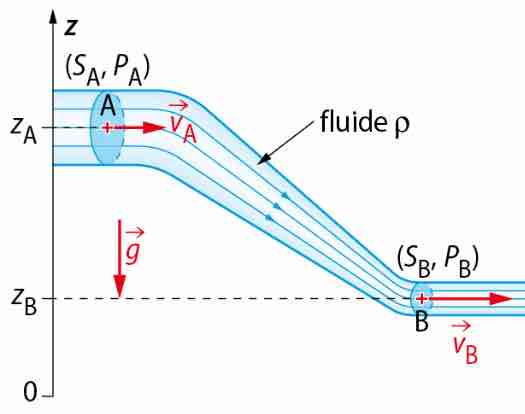
\includegraphics[width=.9\textwidth]{figures/Schema-Bernoulli}  

\end{minipage}

\blocrouge{Énoncé de la relation de Bernoulli}{On considère un fluide parfait, incompressible et en régime permanent.  A et B sont deux points appartenant à une même ligne de courant. On a $$\frac{1}{2}\rho\times  v_A^2 + \rho g z_A + P_A=\frac{1}{2}\rho\times  v_B^2 + \rho g z_B + P_B =cste$$}

\etiquette{Application: Effet Venturi}


Lorsque la variation d'altitude est négligeable. On constate que plus la vitesse du fluide est grande et plus sa pression est petite. Ce résultat s'appelle l'effet Venturi. 

Preuve de l'effet Venturi:

\begin{minipage}{.45\textwidth}
  On veut appliquer la relation de Bernoulli à l'écoulement ci-contre. On admet que  $S_1 >S_2$.
\end{minipage}
\hfill
\begin{minipage}{.55\textwidth}
\includegraphics{figures/venturi}
\end{minipage}
\begin{enumerate}
	\item Ecrire la conservation du débit volumique et en déduire que $v_2>v_1$.
	\item Choisir une ligne de courant avec les points A et B tels que $z_A=z_B$.
	\item Ecrire la relation de Bernoulli le long de la ligne  de courant. 
	\item En déduire que $P_1>P_2$.
\end{enumerate}
L'effet Venturi permet d'expliquer la portance d'une aile d'avion et aussi le fonctionnement d'une trompe à vide (voir exercices)

\begin{travail}
\begin{itemize}
	\item pages 288 à 295
	\item Poussée d'Archimède: 5 , 18 p 288 
	\item Conservation du débit volumique: 9
	\item Relation de Bernoulli: 2 , 17 , 21 , 25 , prepa ECE p 295
	\item Approfondir: 23 , 26
\end{itemize}
\end{travail}
